\documentclass{article}
\usepackage{tikz}

\begin{document}

% \sl diff from \textsl
The general syntax is \\
%$\texttt{.. controls \<\textsl{1st control point}\> and \<\textsl{2nd control point}\> .. \<\textsl{end point}\>}$
%$\texttt{.. controls \textsl{1st control point} and \textsl{2nd control point} .. \textsl{end point}}$
$\small\texttt{.. controls <\textsl{1st control point}> and <\textsl{2nd control point}> .. <\textsl{end point}>}$
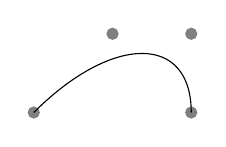
\begin{tikzpicture}
  \filldraw [gray] (0,0) circle [radius=2pt]
                   (1,1) circle [radius=2pt]
                   (2,1) circle [radius=2pt]
                   (2,0) circle [radius=2pt];
  \draw (0,0) .. controls (1,1) and (2,1) .. (2,0);
\end{tikzpicture}
\vspace{1cm}


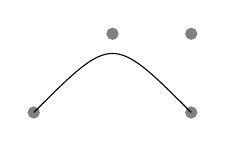
\begin{tikzpicture}
  \filldraw [gray] (0,0) circle [radius=2pt]
                   (1,1) circle [radius=2pt]
                   (2,1) circle [radius=2pt]
                   (2,0) circle [radius=2pt];
  \draw (0,0) .. controls (1,1) .. (2,0);
\end{tikzpicture}
\vspace{1cm}


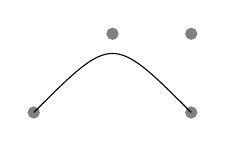
\begin{tikzpicture}
  \filldraw [gray] (0,0) circle [radius=2pt]
                   (1,1) circle [radius=2pt]
                   (2,1) circle [radius=2pt]
                   (2,0) circle [radius=2pt];
  \draw (0,0) .. controls (1,1) and (1,1) .. (2,0);
\end{tikzpicture}







\end{document}






